\scanpage{9}

\uline{\unsure{Suite|Suites} sur l'exponentielle}

\figure{
\begin{tikzpicture}\node[draw,circle,inner sep=4pt] at (0,0) {1};\end{tikzpicture}}
Soit $U$ une Algèbre \inserted{(associative avec unité) linéairement topologique, sép. et complète}
sur $\mathbb Q$, $N(U)$ l'ens de ses éléments top.
nilpotents. On définit deux \uline{bijections} \uline{réciproques}
l'une de l'autre
\diagram{\begin{tikzcd}[ampersand replacement=\&]
N(U)\arrow[r,shift left,"\exp"]\&1_U+N(U)\arrow[l,shift left,"\log"]
\end{tikzcd}}
par
\[
\left\{\begin{aligned}
\exp\deleted{\unsure{\Phi}}\inserted{\xi}&=\sum_{n\ge0}\frac1{n!}\xi^n\\
\log(1+\unsure{\eta|\zeta})&=\sum_{n>0}(-1)^{n+1}\frac1n\unsure{\eta|\zeta}^{n}
\end{aligned}\right.
\]
[N.B. Si la top. de $U$ est discrète, $N$ est l'ens. des \unsure{éléments}
nilpotents].

On a
\diagram{\begin{tikzcd}[column sep=large,ampersand replacement=\&]
\exp(\xi+\xi')=\exp\xi\exp\xi'\&\text{si }[\xi,\xi']=0\arrow[dd,Leftrightarrow]\\
\deleted{\log(1+\xi)(1+\xi')} \& \\
\log gg'=\log g\,\log g'\&\text{si }gg'=g'g
\end{tikzcd}}
\figure{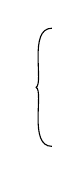
\begin{tikzpicture}\draw(.2,1.5)..controls(-.1,1.5)and(.1,.8)..(0,.75)
..controls(.1,.7)and(-.1,0)..(.2,0);\end{tikzpicture}}

Si \deleted{$\unsure{\varphi U}$} $I$ est un idéal (à gauche ou à droite)
\inserted{fermé} de $U$, on a
\diagram{\begin{tikzcd}[ampersand replacement=\&]
N(U)\cap I\arrow[r,shift left]\&1_U+N(U)\cap I\arrow[l,shift left]
\end{tikzcd}}
\margin{\deleted{$\unsure{P}$}}

Si $\varphi:U\unsure{\text{---}|\to}V$ est un hom d'anneaux \inserted{topologiques},
alors on a $\varphi(N(U))\subset N(V)$, et
\[
\left\{\begin{aligned}
\varphi\exp\xi&=\exp\varphi(\xi)\\
\varphi\log g&=\log\varphi(g)
\end{aligned}\right.
\]
\uline{Cor} \unsure{Toute|Tout} ss-algèbre fermée de $U$ est ``stable'' pour exp, log
\figure{\begin{tikzpicture}[x=1cm,y=1cm]
\draw(.3,4.6)..controls(0,4.7)and(.1,3.6)..(.1,3.4)
..controls(.1,3.2)and(0,2.7)..(.35,2.75);
\draw[->](.12,3.5)..controls(-2,1.2)and(-1.2,-1)..(1.2,-1.1);
\end{tikzpicture}}

\mspage{8}
